\documentclass{standalone}
\usepackage{tikz}
\usetikzlibrary{
  matrix,
  decorations.pathreplacing,
  arrows,
  shapes.geometric
}
\definecolor{blueish}{RGB}{52,152,219}
\definecolor{redish}{RGB}{231,76,60}
\definecolor{greenish}{RGB}{46,204,113}

\begin{document}
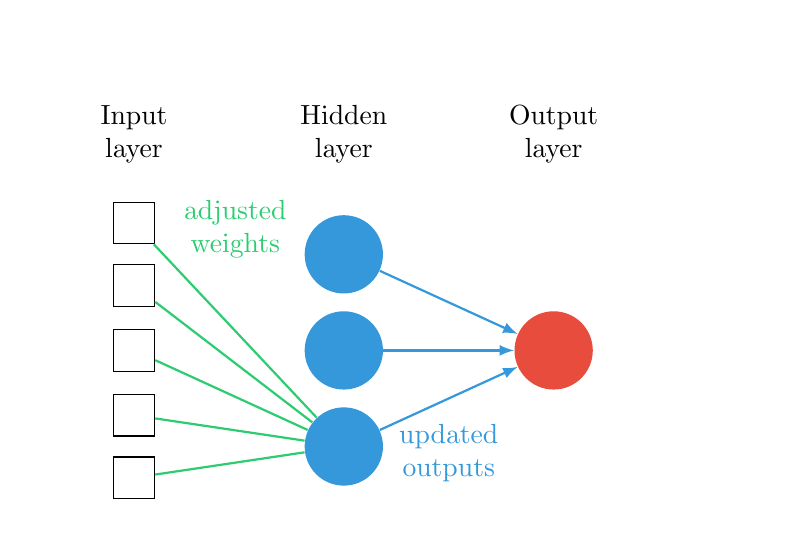
\begin{tikzpicture}[
  plain/.style={
    draw=none,
    fill=none,
  },
  input/.style={
    draw,
    rectangle,
    fill=none,
    minimum width=1.5em,
    minimum height=1.5em,
    inner sep=0pt,
  },
  error/.style={
    draw=none,
    fill=none,
    minimum width=3em,
    minimum height=3em,
    inner sep=0pt,
  },
  nerror/.style={
    draw=none,
    fill=redish
  },
  nweight/.style={
    draw=none,
    fill=blueish
  },
  net/.style={
    matrix of nodes,
    nodes={
      draw,
      circle,
      inner sep=10pt
    },
    nodes in empty cells,
    column sep=0.2cm,
    row sep=-17pt
  },
  >=latex
]

\matrix[net] (mat) {
% Text row
|[plain]| \parbox{1.3cm}{\centering Input\\layer} &
|[plain]| \parbox{1.3cm}{\centering Hidden\\layer} &
|[plain]| \parbox{1.3cm}{\centering Output\\layer} &
|[plain]| \\
% Nodes
|[input]| & |[plain]|   & |[plain]|  & |[plain]|\\
|[plain]| & |[nweight]| & |[plain]|  & |[plain]|\\
|[input]| & |[plain]|   & |[plain]|  & |[plain]|\\
|[plain]| & |[plain]|   & |[plain]|  & |[plain]|\\
|[input]| & |[nweight]| & |[nerror]| & |[error]|\\
|[plain]| & |[plain]|   & |[plain]|  & |[plain]|\\
|[input]| & |[plain]|   & |[plain]|  & |[plain]|\\
|[plain]| & |[nweight]| & |[plain]|  & |[plain]|\\
|[input]| & |[plain]|   & |[plain]|  & |[plain]|\\
};

% Arrows 1
\draw[greenish,thick] (mat-2-1) -- node[above=0.8cm]{\parbox{1.3cm}{\centering adjusted\\weights}} (mat-9-2);
\foreach \ai in {4,6,...,10} {
  \draw[greenish,thick] (mat-\ai-1) -- (mat-9-2);
}


% Arrows 2
\foreach \ai in {3,6} {
  \draw[->,blueish,thick] (mat-\ai-2) -- (mat-6-3);
}
\draw[->,blueish,thick] (mat-9-2) -- node[below=0.2cm]{\parbox{1.3cm}{\centering updated\\outputs}} (mat-6-3);

\end{tikzpicture}
\end{document}
